\section{}
\label{sec:problem2}
%%%%%%%%%%%%%%%%%%%%%%%%%%%%%%%%%%%%%%%%%%%%%%%%%%%%%%%%%%%%%%%%%%%%%%

We consider an area of size $(300 \times 300) \, \si{\meter^2}$ containing a pine tree forest, and the actual locations of the pine trees are to be assessed. The pine tree locations are observed from a satellite by remote sensing, and due to partly cloudy weather the observation probability for individual trees vary across the area.

The area is discretized into a regular $(30 \time 30)$-grid $L$ with grid unit size $\SI{100}{\meter^2}$. The true, but unknown, number of pine trees located in each grid unit is $\{k(x) \ssep x \in L\}$, see figure~\ref{fig:p2_pines}. The probabilities for observing a pine tree in each grid unit is represented by $\{\alpha(x) \ssep x \in L\}$, see figure~\ref{fig:p2_pines}.

\begin{figure}
    \centering
    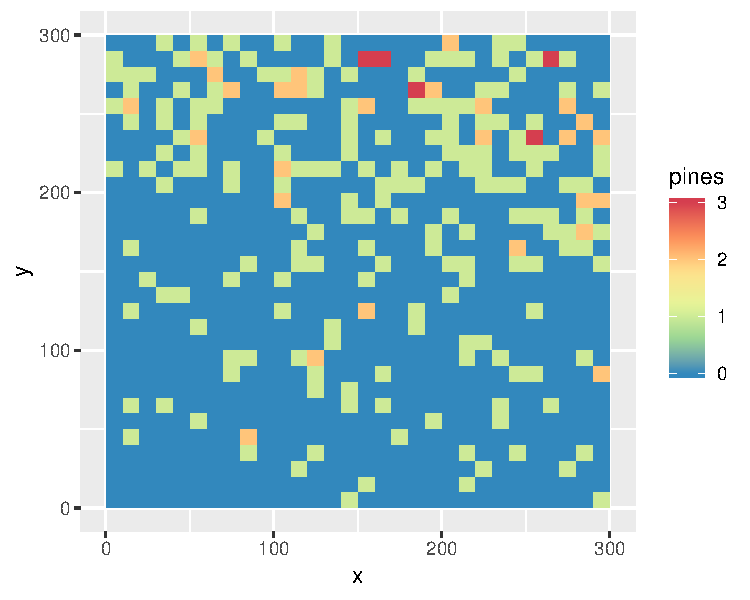
\includegraphics{figures/p2_pines.pdf}
    \caption{Caption}
    \label{fig:p2_pines_plot}
\end{figure}

\begin{figure}
    \centering
    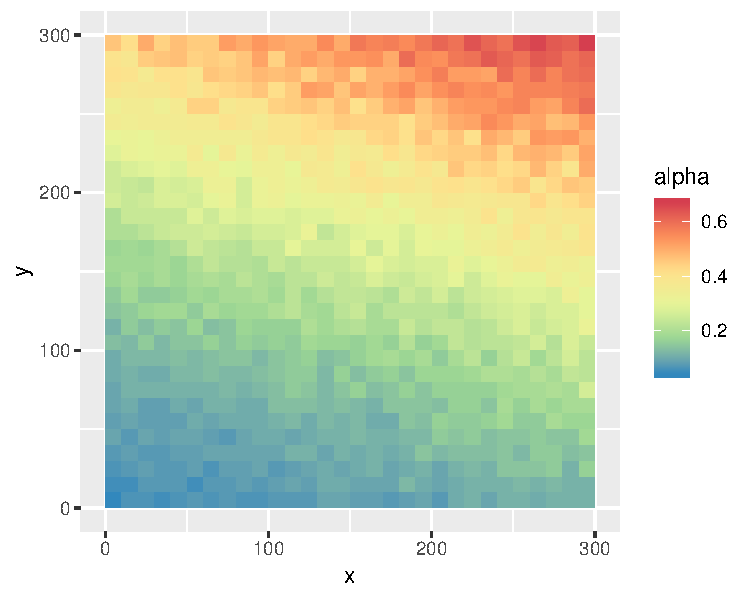
\includegraphics{figures/p2_alpha.pdf}
    \caption{Caption}
    \label{fig:p2_alpha}
\end{figure}